\documentclass{exam}

\usepackage{indentfirst}
\usepackage{graphicx}
\usepackage{listings}
\usepackage{color}
\usepackage{fancyvrb}

\definecolor{mygreen}{rgb}{0,0.6,0}
\definecolor{mygray}{rgb}{0.5,0.5,0.5}
\definecolor{mymauve}{rgb}{0.58,0,0.82}

\lstset{ %
	backgroundcolor=\color{white},		% choose the background color; you must add \usepackage{color} or \usepackage{xcolor}
	basicstyle=\small\ttfamily,		% the size of the fonts that are used for the code
	breakatwhitespace=false,			% sets if automatic breaks should only happen at whitespace
	breaklines=true,					% sets automatic line breaking
	captionpos=b,						% sets the caption-position to bottom
	columns=fullflexible,
	commentstyle=\color{mygreen},		% comment style
	deletekeywords={...},				% if you want to delete keywords from the given language
	escapeinside={\%*}{*)},			% if you want to add LaTeX within your code
	extendedchars=true,				% lets you use non-ASCII characters; for 8-bits encodings only, does not work with UTF-8
	frame=single,						% adds a frame around the code
	keepspaces=true,					% keeps spaces in text, useful for keeping indentation of code (possibly needs columns=flexible)
	keywordstyle=\color{blue},			% keyword style
	language=Octave,					% the language of the code
	morekeywords={*,...},				% if you want to add more keywords to the set
	%   numbers=left,						% where to put the line-numbers; possible values are (none, left, right)
	%   numbersep=6pt,						% how far the line-numbers are from the code
	%   numberstyle=\tiny\color{mygray},	% the style that is used for the line-numbers
	rulecolor=\color{black},			% if not set, the frame-color may be changed on line-breaks within not-black text (e.g. comments (green here))
	showspaces=false,					% show spaces everywhere adding particular underscores; it overrides 'showstringspaces'
	showstringspaces=false,			% underline spaces within strings only
	showtabs=false,					% show tabs within strings adding particular underscores
	stepnumber=1,						% the step between two line-numbers. If it's 1, each line will be numbered
	stringstyle=\color{mymauve},		% string literal style
	tabsize=2,							% sets default tabsize to 2 spaces
	title=\lstname						% show the filename of files included with \lstinputlisting; also try caption instead of title
}

\newcommand{\octavescript}[2]{
	\lstinputlisting[caption=#2,label=#1]{#1}
}

\newcommand{\MNLab}{Laborator\ \#10}
\newcommand{\MNLabTitle}{Transformarea Fourier Rapidă (FFT)}
\newcommand{\MNLabTitleHeader}{FFT}
\newcommand{\MNAuthor}{Andrei STAN, Adelina Vidovici}

\renewcommand{\contentsname}{Cuprins}
\renewcommand{\figurename}{Figura}

\setlength{\parskip}{0.5\baselineskip}

\graphicspath{{./img/}}

\title{
	\textmd{\textbf{\MNLabTitle}}
	\author{Colaboratori: \MNAuthor}
}

\pagestyle{headandfoot}

\header{Metode Numerice}
{\MNLabTitleHeader, Pagina \thepage\ din \numpages}
{2025}
\footer{Facultatea de Automatică și Calculatoare}{}{Pagina \thepage\ din \numpages}

\begin{document}

\begin{coverpages}

	\maketitle
	\tableofcontents

\end{coverpages}

\section{Obiective laborator}

În urma parcurgerii acestui laborator, studentul va fi capabil să:

\begin{itemize}
	\item Determine polinomul de interpolare trigonometrică folosind tehnica de calcul directă;
	\item Aplice transformarea Fourier rapidă pentru a determina polinomul de interpolare trigonometrică;
\end{itemize}

%----------------------------------------------------------------------------------------
%       TEORIE
%----------------------------------------------------------------------------------------

\section{Noțiuni teoretice}

\subsection{Transformarea Fourier rapidă}

Interpolarea unui set de date alcătuit din $2m$ puncte folosind tehnica de calcul directă necesită efectuarea unui număr mare de operații (aproximativ $(2m)^{2}$ operații de înmulțire și $(2m)^{2}$ operații de adunare), motiv pentru care și eroarea obținută în cazul unui număr mare de puncte este foarte mare.


Tehnica de calcul directă presupune determinarea polinomului de interpolare trigonometrică pentru cele $2m$ puncte ${(x_j, y_j)}$, cu $x_j = -\pi + (j/m)\pi$, pentru oricare $j = 0, 1, ..., 2m-1$ folosind  formula următoare:
$$S_m(x) = \frac{a_0 + a_m\cos mx}{2} + \sum_{k=0}^{m-1} (a_k\cos kx + b_k\sin kx)$$
unde:
\begin{itemize}
	\item$a_k = \frac{1}{m}\sum_{j=0}^{2m-1} y_j\cos kx_j$, pentru oricare $k=0, 1, ..., m$
	\item$b_k = \frac{1}{m}\sum_{j=0}^{2m-1} y_j\sin kx_j$, pentru oricare $k=1, 2, ..., m-1$
\end{itemize}

Metoda alternativă de a determina forma polinomului de interpolare trigonometrică necesită  $O(m\log_2 m)$ operații de înmulțire și $O(m\log_2 m)$ operații de adunare. Astfel, numărul de operații necesare pentru obținerea polinomului de interpolare trigonometrică devine de ordinul miilor, atunci când setul de date este de ordinul miilor, spre deosebire de calculul direct unde numărul de operații este de ordinul milioanelor.

Metoda poartă numele de transformata Fourier rapidă (Fast Fourier Transform). În locul evaluării directe a constantelor $a_k$ și $b_k$, transformarea Fourier rapidă modifică valoarea coeficienților complecși $c_k$ în:
$$\frac{1}{m}\sum_{j=0}^{2m-1} c_ke^{ikx}$$
unde $c_k = \sum_{j=0}^{2m-1} y_je^{ik\pi j/m}$, pentru oricare $k = 0, 1, ..., 2m-1$.

Odată constantele $c_k$ determinate, $a_k$ și $b_k$ pot fi calculate folosind formula lui \textit{Euler}: $e^{iz} = \cos z + i\sin z.$

În plus, pentru orice valoare întreagă a lui $n$:
\begin{center}
	$e^{n\pi i} = \cos n\pi + i\sin n\pi = (-1)^{n}.$
\end{center}
astfel încât $a_k + ib_k = \frac{(-1)^{k}}{m}c_k$, cu precizarea că atât $b_0$ și $b_m$ sunt egale cu $0$ și nu contribuie la rezultatul final.

Presupunând că $m = 2^p$ (m este o putere a lui 2), pentru orice $k = 0, 1, ..., m-1$, vom avea:
$$c_k + c_{k+m}= \sum_{j=0}^{2m-1} y_je^{ik\pi j/m} + \sum_{j=0}^{2m-1} y_je^{i(k+m)\pi j/m} = \sum_{j=0}^{2m-1} y_je^{ik\pi j/m}(1 + e^{\pi ij}).$$

Dar
$$1 + e^{\pi ij} =
	\left\{
	\begin{array}{ll}
		2 & \mbox{dacă j este par}   \\
		0 & \mbox{dacă j este impar}
	\end{array}
	\right.$$
ceea ce înseamnă că doar $m$ termeni sunt diferiți de $0$ și contribuie la rezultatul final.

Dacă înlocuim indicele $j$ cu $2j$ atunci când scriem suma, vom obține:
$$c_k + c_{k+m}= 2\sum_{j=0}^{m-1} y_{2j}e^{ik\pi (2j)/m},$$
echivalent cu relația:
$$c_k + c_{k+m}= 2\sum_{j=0}^{m-1} y_{2j}e^{ik\pi j/(m/2)}.$$

În mod similar,
$$c_k - c_{k+m}= 2e^{ik\pi /m}\sum_{j=0}^{m-1} y_{2j+1}e^{ik\pi j/(m/2)}$$

Atât $c_k$ și $c_{k+m}$ pot fi determinate din cele două relații. Procesul va lua sfârșit după $p + 1$ iterații.

%----------------------------------------------------------------------------------------
%	PROBLEM 1
%----------------------------------------------------------------------------------------
\section{Probleme rezolvate}

\subsection{Problema 1}
Aplicați transformarea Fourier rapidă asupra unui set de $8 = 2^3$ puncte $(x_j, y_j)$, unde $x_j = -\pi + j\pi/4$, cu $j = 0, 1, ..., 7$. Comparați numărul de operații folosite în cadrul tehnicii de calcul directe a polinomului de interpolare trigonometrică cu numărul de operații necesare în cadrul transformării Fourier rapide.

\textit{Soluție:}

În acest caz, $2m = 8$, deci $m = 4 = 2^2$ și $p = 2$.

$S_4(x) = \frac{a_0 + a_4\cos 4x}{2} + \sum_{k=1}^{3} (a_k\cos kx + b_k\sin kx)$, unde

$a_k = \frac{1}{4}\sum_{j=0}^{7} y_j\cos kx_j$ și $b_k = \frac{1}{4}\sum_{j=0}^{7} y_j\sin kx_j$, pentru oricare $k=0, 1, 2, 3, 4.$

Definim transformarea Fourier ca fiind:

$\frac{1}{4}\sum_{j=0}^{7} c_ke^{ikx},$
unde $c_k = \sum_{j=0}^{7} y_je^{ik\pi j/4}$, pentru $k = 0, 1, ..., 7$.

Pentru a determina constantele $a_k$ și $b_k$ vom folosi relația $a_k + ib_k = \frac{1}{4}e^{-ik\pi}c_k.$

Folosind calculul direct, obținem constantele $c_k$:

$c_0 = y_0 + y_1 + y_2 + y_3 + y_4 + y_5 + y_6 + y_7$

$c_1 = y_0 + (\frac{i+1}{\sqrt{2}})y_1 + iy_2 + (\frac{i-1}{\sqrt{2}})y_3 - y_4 - (\frac{i+1}{\sqrt{2}})y_5 - iy_6 - (\frac{i-1}{\sqrt{2}})y_7$

$c_2 = y_0 + iy_1 - y_2 - iy_3 + y_4 + iy_5 - y_6 - iy_7$

$c_3 = y_0 + (\frac{i-1}{\sqrt{2}})y_1 - iy_2 + (\frac{i+1}{\sqrt{2}})y_3 - y_4 - (\frac{i-1}{\sqrt{2}})y_5 + iy_6 - (\frac{i+1}{\sqrt{2}})y_7$

$c_4 = y_0 - y_1 + y_2 - y_3 + y_4 - y_5 + y_6 - y_7$

$c_5 = y_0 - (\frac{i+1}{\sqrt{2}})y_1 + iy_2 - (\frac{i-1}{\sqrt{2}})y_3 - y_4 + (\frac{i+1}{\sqrt{2}})y_5 - iy_6 + (\frac{i-1}{\sqrt{2}})y_7$

$c_6 = y_0 - iy_1 - y_2 + iy_3 + y_4 - iy_5 - y_6 + iy_7$

$c_7 = y_0 - (\frac{i-1}{\sqrt{2}})y_1 - iy_2 - (\frac{i+1}{\sqrt{2}})y_3 - y_4 + (\frac{i-1}{\sqrt{2}})y_5 + iy_6 + (\frac{i+1}{\sqrt{2}})y_7$

Pentru că, în acest caz, setul de date este unul mic, mulți dintre coeficienții termenilor $y_i$ sunt egali cu $1$ sau cu $-1$. Pentru a putea compara număr de operații necesare, vom lua în considerare și înmulțirile cu $1$ și cu $-1$. Astfel, sunt necesare $64$ de înmultiri/împărțiri și $56$ operații de adunare/scădere pentru obținerea constantelor $c_0, c_1, ..., c_7$ folosind calculul direct.

Pentru a determina primul pas din transformarea Fourier rapidă, vom defini:

$d_0 = \frac{c_0 + c_4}{2} = y_0 +  y_2 + y_4 + y_6$

$d_1 = \frac{c_0 - c_4}{2} = y_1 +  y_3 + y_5 + y_7$

$d_2 = \frac{c_1 + c_5}{2} = y_0 +  iy_2 - y_4 - iy_6$

$d_3 = \frac{c_1 - c_5}{2} = (\frac{i+1}{\sqrt{2}})(y_1 +  iy_3 - y_5 - iy_7)$

$d_4 = \frac{c_2 + c_6}{2} = y_0 -  y_2 + y_4 - y_6$

$d_5 = \frac{c_2 - c_6}{2} = i(y_1 -  y_3 + y_5 - y_7)$

$d_6 = \frac{c_3 + c_7}{2} = y_0 -  iy_2 - iy_4 + iy_6$

$d_7 = \frac{c_3 - c_7}{2} = (\frac{i-1}{\sqrt{2}})(y_1 -  iy_3 - y_5 + iy_7)$

Pentru cel de-al doilea pas din transformarea Fourier rapidă, vom defini:

$e_0 = \frac{d_0 + d_4}{2} = y_0 +  y_4$

$e_1 = \frac{d_0 - d_4}{2} = y_2 +  y_6$

$e_2 = \frac{id_1 + d_5}{2} = i(y_1 +  y_5)$

$e_3 = \frac{id_1 - d_5}{2} = i(y_3 +  y_7)$
$e_4 = \frac{d_2 + d_6}{2} = y_0 - y_4$

$e_5 = \frac{d_2 - d_6}{2} = i(y_2 - y_6)$

$e_6 = \frac{id_3 + d_7}{2} = (\frac{i-1}{\sqrt{2}})(y_1 - y_5)$

$e_7 = \frac{id_3 - d_7}{2} = i(\frac{i-1}{\sqrt{2}})(y_3 - y_3)$

Cel de-al treilea pas $(3 = p + 1)$ al transformării presupune definirea:

$f_0 = \frac{e_0 + e_4}{2} = y_0$

$f_1 = \frac{e_0 - e_4}{2} = y_4$

$f_2 = \frac{ie_1 + e_5}{2} = iy_2$

$f_3 = \frac{ie_1 - e_5}{2} = iy_6$

$f_4 = \frac{(\frac{i+1}{\sqrt{2}})e_2 + e_6}{2} = (\frac{i-1}{\sqrt{2}})y_1$

$f_5 = \frac{(\frac{i+1}{\sqrt{2}})e_2 - e_6}{2} = (\frac{i-1}{\sqrt{2}})y_5$

$f_6 = \frac{(\frac{i-1}{\sqrt{2}})e_3 + e_7}{2} = (\frac{-i-1}{\sqrt{2}})y_3$

$f_7 = \frac{(\frac{i-1}{\sqrt{2}})e_3 - e_7}{2} = (\frac{-i-1}{\sqrt{2}})y_7$

Valorile $c_0, c_1, ..., c_7$, $d_0, d_1, ..., d_7$, $e_0, e_1, ..., e_7$, $f_0, f_1, ..., f_7$ sunt independente de setul de puncte şi depind doar de valoarea lui $m = 4$. Pentru fiecare valoare $m$, există un set unic de constante $c_k$, $d_k$, $e_k$, $f_k$, cu $k = 0, 1, ...7$. Calculele anterioare nu sunt neapărat necesare în cadrul unei aplicații.

În cele ce urmează vom prezenta calculele necesare pentru determinarea polinomului de interpolare trigonometrică folosind transformata Fourier rapidă:

Determinarea valorilor $f_k$:

$f_0 = y_0;    f_1 = y_4;    f_2 = iy_2;    f_3 = iy_6;$

$f_4 = (\frac{i-1}{\sqrt{2}})y_1;$   $f_5 = (\frac{i-1}{\sqrt{2}})y_5;$   $f_6 = (\frac{-i-1}{\sqrt{2}})y_3;$   $f_7 = (\frac{-i-1}{\sqrt{2}})y_7;$

Determinarea valorilor $e_k$:

$e_0 = f_0 + f_1;    e_1 = -i(f_2 + f_3);    e_2 = (\frac{i-1}{\sqrt{2}})(f_4 + f_5);    e_3 = -(\frac{i+1}{\sqrt{2}})(f_6 + f_7);$

$e_4 = f_0 - f_1;$   $e_5 = f_2 - f_3;$   $e_6 = f_4 - f_5;$   $e_7 = f_6 - f_7;$

Determinarea valorilor $d_k$:

$d_0 = e_0 + e_1;    d_1 = -i(e_2 + e_3);    d_2 = e_4 + e_5;    d_3 = -i(e_6 + e_7);$

$d_4 = e_0 - e_1;$   $d_5 = e_2 - e_3;$   $d_6 = e_4 - e_5;$   $d_7 = e_6 - e_7;$

Determinarea valorilor $c_k$:

$c_0 = d_0 + d_1;    c_1 = d_2 + d_3;    c_2 = d_4 + d_5;    c_3 = d_6 + d_7;$

$c_4 = d_0 - d_1;$   $c_5 = d_2 - d_3;$   $c_6 = d_4 - d_5;$   $c_7 = d_6 - d_7;$

Analizând numărul de operații necesare în acest caz, vom obține $24$ de înmulțiri/împărțiri și $24$ de operații de adunare/scădere.
%\end{Problem}

\subsection{Problema 2}
Scrieţi un program OCTAVE care să calculeze valoarea polinomului de interpolare trigonometrică  $S_m(x)$ pentru $x = x_0$, funcţia $f(x) = x^2 + x + 1$,  pe intervalul  $[ -\pi, \pi]$. Se va folosi tehnica de calcul directă. Programul primeşte ca parametrii de intrare: $m$, unde $2m$ este numărul de puncte din setul de date, $x_0$ şi funcţia $f$.

\textit{Soluție:}

\octavescript{./src/PolinomTrigonometric.m}{Funcţie pentru calcularea polinomului de interpolare trigonometrică.}

Pentru testarea programului, puteţi folosi următoarea secvenţă:
\octavescript{./src/testare.m}{Fişier de testare.}

iar rezultatul este:

\begin{figure}[ht]
	\begin{center}
		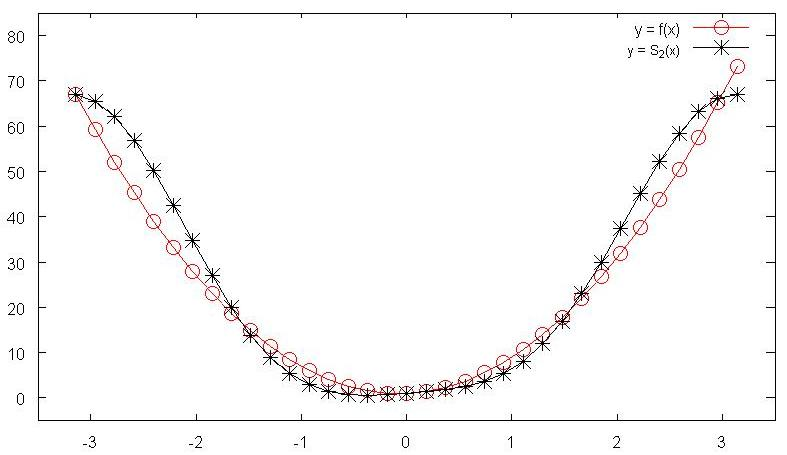
\includegraphics[width=139mm]{./img/poltrigo} % Example image
		\caption{Graficul rezultat pentru fişierul de testare.}
	\end{center}
	\label{metoda pozitiei false}
\end{figure}

%----------------------------------------------------------------------------------------
\section{Probleme propuse}

\subsection{Problema 1}
Implementați în OCTAVE algoritmul de determinare al polinomului de interpolare trigonometrică pentru $2m$ puncte ${(x_j, y_j)}$, cu $x_j = -\pi + (j/m)\pi$, pentru oricare $j = 0, 1, ..., 2m-1$, folosind transformarea Fourier rapidă.  Datele de intrare sunt: $m$ putere a lui $2$, unde $2m$ este numărul de puncte din setul de date; valorile $y_0$, $y_1$, ..., $y_{2m-1}$. Datele de ieșire sunt: valorile complexe $c_0$, $c_1$, ..., $c_{2m-1}.$

%\end{Problem}

\subsection{Problema 2}
Determinați polinomul de interpolare trigonometrică de grad $5$, pe intervalul $[0, 3]$, pentru setul de date $(j/5, f(j/5))$ cu $j = 0, 1, ..., 9$, unde:
$$f(x) =  4x^3 - x^2 + \tan (x-1).$$

%\end{Problem}

\end{document}
